\section{Reproducible evidence and performance measurements}
\label{sec:experiments}

\subsection{Native corpus and comparison discipline}

The final audit uses 106 retained historical source cases and a 14-case
extension containing interior vertices and source three-handles. This is a
normal-cut corpus, with reducible test manifolds as well as knot exteriors and
solid tori. It is not a random sample of knot diagrams or a whole-recognizer
benchmark. Every input triangulation and normal vector is copied into the
package. Seven cases have binary disk counts beyond the explicit 4096-disk
oracle cap; the largest uses a 16385-bit nonzero coordinate.

Three producers are evaluated on each source: the current canonical default,
the new direct group terminal, and the independently loaded incoming
deferred-forest overlay. All their positive outputs are independently replayed.
Table~\ref{tab:coverage} gives the final counts. The two portfolio rows are
unions of independently obtained positive certificates; they do not claim a
new jointly optimized schedule.

\begin{table}[htbp]
\centering
\begin{tabular}{lrrr}
\toprule
Method & Historical / 106 & Interior / 14 & Total / 120 \\
\midrule
Current canonical default & 92 & 12 & 104 \\
New group terminal alone & 64 & 12 & 76 \\
Deferred-forest comparison & 99 & 12 & 111 \\
Canonical plus group & 95 & 12 & 107 \\
Deferred plus group & 100 & 12 & 112 \\
\bottomrule
\end{tabular}
\caption{Fresh source-bound whole-cut handlebody certificates. A refusal is inconclusive.}
\label{tab:coverage}
\end{table}

The older incoming article had 102 canonical positives. At the present pinned
revision the default already solves \code{interior\_loop/empty} and
\code{interior\_loop/boundary\_link}, bringing that baseline to 104. These two
are not credited to the new contribution. The new group terminal adds
\code{pilot/finite\_trefoil/0}, \code{pilot/finite\_figureEight/0} and
\code{pachner23\_5\_8\_2/mixed} beyond the current default. Only the figure-eight
case is new beyond the deferred method.

There are 291 independently replayed positive producer outputs in the audit:
$104+76+111$. All 76 new group positives additionally retain complete serialized
packets that were replayed from their delivered JSON files. A fresh literal
Regina~\cite{Regina} cut and component recognition completed on 113 inputs, with no oracle
timeout. The remaining seven were deliberately not expanded. The agreement
counts are 97 canonical, 69 new group and 104 deferred; the portfolio agrees on
all 105 explicit oracle-positive cases. Each of the eight portfolio refusals
has an oracle component recognized as nonhandlebody. This describes the finite
corpus only and provides no completeness guarantee on unseen sources.

The audit harness initially compared one decoded huge integer with its equal
hexadecimal transport string and reported a false disagreement at the 106th
case. The integer-field comparison was corrected, and the final 15 cases were
run after a hash guard verified all production sources, fixtures and deferred
files against the retained first 105. No source or algebraic checker failed.
The final report and methodology preserve that recovery rather than presenting
the first invocation as uninterrupted. The corrected script can reproduce the
whole audit from scratch.

\subsection{The Euler gate detects real omitted topology}

The disk-base compiler admits 83 of the 120 sources. Of these, 76 obtain a
complete handlebody certificate, two stall in the final deterministic word
policy, and five have completely free presentations but fail the Euler gate.
The other 37 sources contain a nondisk base and are outside this compiler's
contract.

For all five Euler failures, the package separately retains and replays the
authenticated source presentation and every completed component group trace.
Table~\ref{tab:defects} gives their exact values. The fixture names refer to
the saved source cases, and do not assert that a closed manifold itself was
fed to the torus-boundary validator. The theorem computes the topology of the
corresponding whole cut.

\begin{table}[htbp]
\centering\small
\begin{tabular}{P{0.48\linewidth}rrrrrr}
\toprule
Source fixture & $\chi$ & $c$ & $r$ & $z$ & $h_3$ & $b_2$ \\
\midrule
\path{pilot/solid_torus_sum_s2xs1/0} & 1 & 1 & 1 & 1 & 0 & 1 \\
\code{interior\_2\_3/mixed} & 3 & 3 & 1 & 2 & 1 & 1 \\
\path{solid_torus_sum_s2xs1/mixed} & 3 & 3 & 2 & 2 & 0 & 2 \\
\path{nested_1_4_6/interior_links} & 12 & 7 & 1 & 12 & 6 & 6 \\
\code{interior\_loop/interior\_links} & 2 & 2 & 1 & 2 & 1 & 1 \\
\bottomrule
\end{tabular}
\caption{Independently replayed free-group sources with $b_2=\chi-c+r=z-h_3>0$.}
\label{tab:defects}
\end{table}

These cases justify retaining the original three-handles and source Euler
characteristic even when the group simplifier deletes all relators. A terminal
rule that identified a free group with a handlebody without the topological
gate would give incorrect answers on this retained corpus.

\subsection{Independent algebraic audit and regression suite}

A separate algebraic audit examines 10203 presentations. It includes all 1365
one-relator presentations on two generators through length five, all 7225
ordered pairs of relators through length three, 1600 deterministic random
signed presentations with sparse labels, named nonfree and incomplete free
examples, empty edge cases, and the two figure-eight components. The seed and
source hashes are retained.

The producer completes 6748 cases and refuses 3455. Each success is checked by
an independent explicit-map implementation: it derives the solved generator
from the equation $p x^\varepsilon q=1$, verifies conjugations used by cyclic
reduction, and tracks original generators into the final free group. Original
relators must vanish and surviving generators must map identically. Its word
oracle repeatedly deletes adjacent inverse pairs rather than importing either
production stack reducer.

There are also 481 exhaustive nonabelian $S_3$ homomorphism-count comparisons,
485 separate Regina group recognitions, and 3240 rejected certificate mutations.
For a claimed $F_r$, the $S_3$ homomorphism count must be $6^r$; this is an
additional check, not a proof of freeness. The exact Tietze trace supplies that
proof. Both automorphism examples on which the policy stalls are included.

The integrated native regression run passes all 1749 tests. A separate run of
the 33 new focused tests passes as well. They exercise source-word orientation,
loop one-handles, interval-cycle free factors, three-handles, huge integers,
producer-disabled replay, hostile certificates, old default compatibility,
budgets and callback propagation. The raw logs are included. No formal proof
assistant certification is claimed.

\subsection{Measured query cost}

Measurements were run after the concurrent regression and audit jobs had
finished. Each case uses one warm-up per arm followed by seven randomized-order
rounds. Two identical new-terminal arms provide an A/A control. Imports and
process startup are outside the measured intervals. Each native arm includes
source construction, proof production, JSON serialization/deserialization and
independent source replay. Regina includes triangulation and surface import,
literal cutting, component recognition and result serialization. Thus the
comparison asks for the same unmarked genus census, with the native path also
delivering an independently replayed certificate. A refusal is retained as a
different outcome and never counted as a faster successful recognition.

The three newly covered native cases test the actual added capability. A
one-tetrahedron meridian family separately illustrates dependence on represented
weight; that compression benefit already exists in the preceding native
infrastructure and is not attributed solely to the new group reducer. Seven
rounds provide descriptive local measurements, not a distributional runtime
guarantee. Raw samples, A/A ratios, versions and source hashes accompany the
derived table.

\begin{table}[htbp]
\centering\small
\begin{tabular}{lrrrr}
\toprule
Case & Group ms & Portfolio ms & Regina ms & Literal tets \\
\midrule
Trefoil cut & 5.66 & 5.72 & 24.71 & 122 \\
Figure-eight cut & 75.46 & 110.09 & 22.47 & 319 \\
Mixed Pachner cut & 1251.63 & 2064.32 & 3.18 & 283 \\
One meridian copy & 1.83 & 1.80 & 0.39 & 31 \\
64 meridian copies & 7.40 & 7.54 & 5.87 & 850 \\
1024 meridian copies & 8.40 & 7.99 & 111.28 & 13330 \\
$2^{128}$ copies & 8.11 & 8.63 & --- & --- \\
$2^{500}$ copies & 8.37 & 8.69 & --- & --- \\
$2^{16384}$ copies & 35.24 & 36.79 & --- & --- \\
\bottomrule
\end{tabular}
\caption{Median complete-query costs in milliseconds, seven rounds. Group uses arm A; the two identical A/A arms are retained in the raw data. Dashes denote the expansion cap. The mixed Pachner row is from the separately retained completed retry.}
\label{tab:timings}
\end{table}


For the trefoil cut, the new complete certified query takes about 5.7 ms versus
24.7 ms for the literal Regina task. For the figure-eight cut it takes about
75.5 ms versus 22.5 ms. The mixed Pachner case is a substantial regression:
about 1.25 seconds for the direct certified query and 2.06 seconds with the
failed geometric fast path, versus about 3.18 ms for Regina. Its active group
presentation has only 27 letters; the complete source/proof pipeline remains
an important practical cost. These comparisons include the different proof
deliverables described above and must not be promoted to universal speed
claims.

The mixed case exceeded the original aggregate 45-second cap for all warm-ups
and repeated arms. The same seven-round worker was rerun separately and
completed; both the original timeout and the completed raw samples are retained.
Across the displayed cases, median ratios of the identical A/A arms range
from about 0.91 to 1.10, indicating material timing variability. On 1024
meridian copies the direct certified query takes about 8.4 ms versus 111 ms for
the literal task, but most of that advantage is inherited binary compression.
For $2^{16384}$ copies the group query is about 35 ms; the explicit task is
not attempted, and its cost is not extrapolated.

A single separately retained cProfile run attributes 98.4\% of its instrumented
wall time to four disjoint inherited stages: parallelity source production,
moment-boundary production, and their independent replayers. The new finite
compiler, group reducer and corresponding finite checkers together account for
about 0.086\% under that profiler. Source-proof fields occupy 384724 of the
387809 compact certificate bytes. These are diagnostic attributions, not
unprofiled timing estimates. In particular, reducing the 27-letter algebraic
trace cannot repair the measured full-query regression by itself.

The profile records 1161 calls both to source interval contraction and to the
weighted verifier's prefix-event reconstruction, with 884 translation folds.
This suggests two concrete targets: independently checked incremental support
and prefix structures, and an explicit orbit path guarded by a polynomial
bound on universe size. Appendix~\ref{sec:bounded-expansion} proves that the
latter design can preserve binary-input complexity guarantees. Neither source
optimization is included in the present production patch.

\begin{figure}[htbp]
\centering
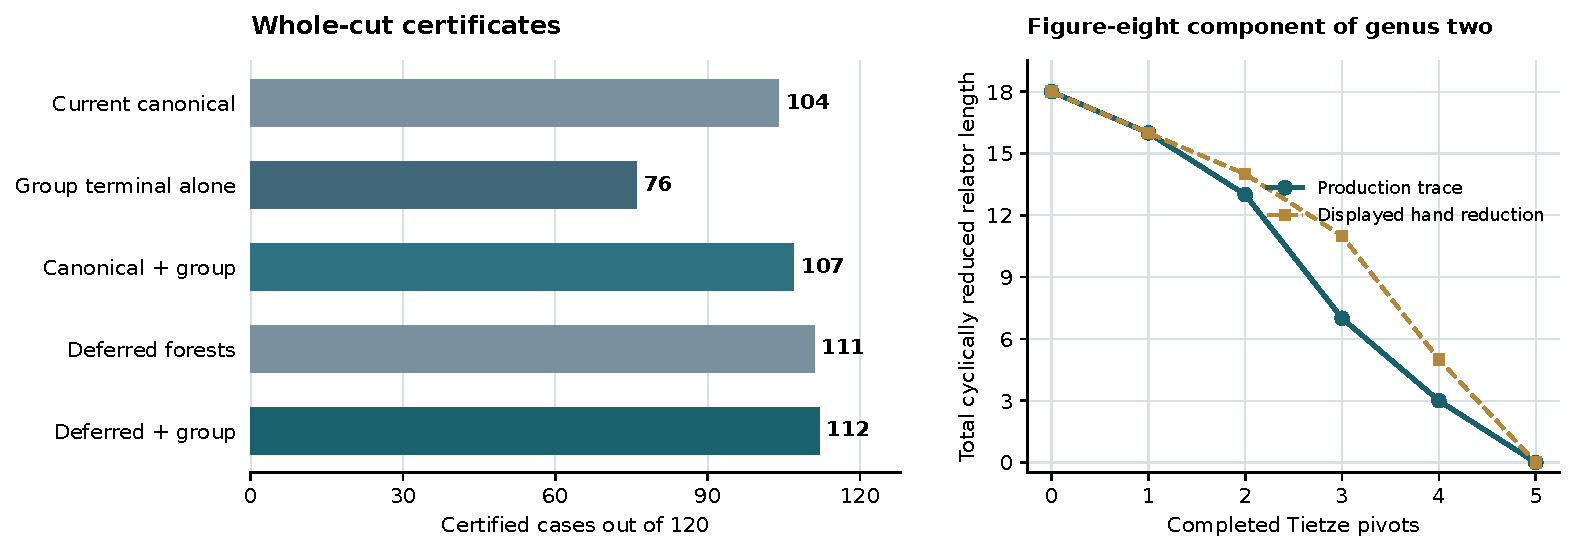
\includegraphics[width=\linewidth]{figures/coverage_and_trace.pdf}
\caption{Left: certified whole-cut coverage on the retained 120 cases.
Right: exact accepted relator lengths for the difficult figure-eight
component. Coverage and word lengths are exact counts, not timing estimates.}
\label{fig:coverage-trace}
\end{figure}

The practical integration decision is therefore conservative: preserve the
geometric fast path and expose the group terminal as an opt-in fallback.
Its main new value is additional certified coverage and a finite algebraic
terminal interface. Latency improvements depend on the surrounding scheduler
and which expensive alternatives the new certificate avoids.
